\documentclass{article} 
\usepackage{graphicx} % Required for inserting images
\usepackage[a4paper, left=2cm, right=2cm, top=2cm, bottom=2cm]{geometry}
\usepackage{tikz}
\usepackage{amsmath, amssymb}
\usepackage{fancyhdr}
\usepackage{helvet} 
\usepackage{lmodern}

\pagestyle{fancy}
\fancyhf{}

\fancyhead[L]{Student : Kuldeep(23684)}  % Left side
\fancyhead[C]{AI-ML (UMC203)}               % Centered
\fancyhead[R]{Instructor : Chiranjib Bhattacharyya}           % Right side

\begin{document}
    \thispagestyle{empty}
    \begin{center}
        \huge{\textbf{Artificial Intelligence and Machine Learning}} \\ 
        \vspace{1cm}
        \huge{\textbf{Assignment 02}} \\ 
        \vspace{2cm}
        \huge{\textbf{Instructor : Prof. Chiranjib Bhattacharyya}} \\
        \vspace{0.5cm}
        \huge{\textbf{Student : Kuldeep Jatav}} \\
        \vspace{0.5cm}
        \huge{\textbf{SR Number: 23684}} \\ 
        \vspace{3cm}

        
\includegraphics[width=0.5\textwidth]{IIScLogo.jpg}
    \end{center}
    
    \newpage
\noindent    \textbf{Solution 1 : Support Vector Machine and Perceptron}
\begin{itemize}
    \item \textbf{Tasks}
    
    \textbf{1.} Perceptron algorithm does not seem converging on the given dataset maybe the dataset is not linearly separable, to be more sure i ran the perceptron algorithm for 100000 iterations still the lowest misclassification rate achieved was around 0.193, and in the next part when we remove the points which are causing non-separability the algorithm converged in $\approx$ 300 iterations

    \textbf{2.} Slack support vector machine with linear kernel
    \begin{itemize}
        \item Primal version
        \[
        \min_{\mathbf{w}, b, \boldsymbol{\xi}} \quad \frac{1}{2} \|\mathbf{w}\|^2 + C \sum_{i=1}^{n} \xi_i
        \]
        \hspace{60pt} subject to
        \[
        y_i (\mathbf{w}^T \mathbf{x}_i + b) \geq 1 - \xi_i, \quad \forall i = 1, \dots, n
        \]
        \[
        \xi_i \geq 0, \quad \forall i = 1, \dots, n
        \]
        \item Dual version
        \[
        \max_{\boldsymbol{\alpha}} \quad \sum_{i=1}^{n} \alpha_i - \frac{1}{2} \sum_{i=1}^{n} \sum_{j=1}^{n} \alpha_i \alpha_j y_i y_j \mathbf{x}_i^T \mathbf{x}_j
        \]
        \hspace{60pt} subject to
        \[
        0 \leq \alpha_i \leq C, \quad \forall i = 1, \dots, n
        \]

        \[
        \sum_{i=1}^{n} \alpha_i y_i = 0
        \]
        while solving both problems i used \textbf{cvxopt} for convex optimization with $C=1$ 
    \end{itemize}
        \textbf{3.} In this part i used Gaussian kernel with $\gamma = 0.1$ and $C=1.0$
        \[K(x,z) = exp\left(- \frac{|| x-z ||^2}{2 \sigma ^ 2} \right) \hspace{10pt},\hspace{10pt} \gamma = \frac{1}{2\sigma^2}\]

        \textbf{4.} In this part first i make $new\_data$ by removing the points which were causing non-separability and then again ran the perceptron algorithm on this new data it converged in $\approx$ 300 iterations
    \item \textbf{Deliverables}
    
    \textbf{1.} Plot of misclassification rate vs number of iterations for perceptron algorithm on given dataset
    \begin{figure}[h]
        \centering
        \begin{minipage}{0.45\textwidth}
            \centering
            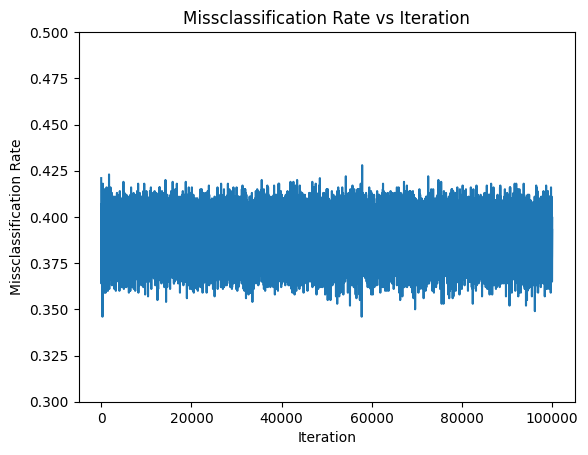
\includegraphics[width=\linewidth]{non_convergence_misclassification_vs_iterations.png}
            \caption{$\mathbf{10^5}$ \textbf{ Iterations}}
        \end{minipage}
        \hfill
        \begin{minipage}{0.45\textwidth}
            \centering
            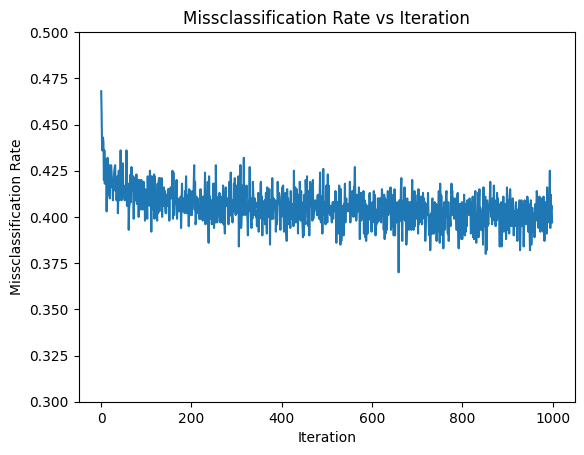
\includegraphics[width=\linewidth]{non_convergence_misclassification_vs_1000iterations.png}
            \caption{$\mathbf{10^3}$ \textbf{ Iterations}}
        \end{minipage}
        \caption{Two adjacent images}
    \end{figure}

\newpage
    \textbf{2.} For the given dataset so dual version is faster than primal version because 
    \begin{itemize}
        \item Primal time : $\approx 1.24$  \texttt{seconds}
        \item Dual time : $\approx 1.17$  \texttt{seconds}
    \end{itemize}

    \textbf{3.} For images that cause non-separability refer \boxed{\texttt{inseparable\_23684.csv}} (attached in submission).

    \textbf{4.} Final misclassification rate for the kernelized SVM 
    \begin{itemize}
        \item 145 out of 1000 train points were misclassified
        \item 19 out of 200 test points were misclassified
    \end{itemize}

    \textbf{5.} plot of misclassification rate vs number of iterations for perceptron algorithm on given dataset after removing the points which were causing non-separability
    \begin{figure}[h]
        \centering
        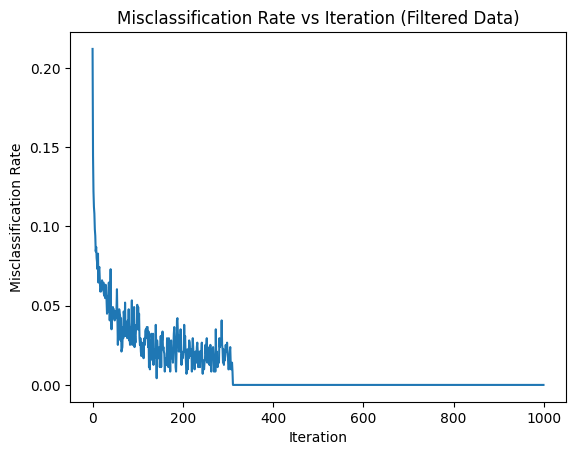
\includegraphics[width=0.5\textwidth]{convergence_misclassification_vs_iterations.png}
        \caption{Misclassification rate vs number of iterations}
    \end{figure}
\end{itemize}

\noindent    \textbf{Solution 2 : Logistic Regression, MLP, CNN \& PCA}
\begin{itemize}
    \item \textbf{Tasks}
    
    \textbf{1.} In this part we constructed an MLP model with following architecture
    \begin{itemize}
        \item Input layer : 784 neurons
        \item Hidden layer 1 : 512 neurons with ReLU activation
        \item Hidden layer 2 : 256 neurons with ReLU activation
        \item Output layer : 10 neurons with softmax activation
        \item Loss function : Cross entropy loss
    \end{itemize}
    On running the code for 20 epochs with \textbf{80:20} split then i got $\approx$ 94\% accuracy on test data

\hspace{15pt}

    \textbf{2.} In this part i constructed a CNN model that takes $28 \times 28$ as input \& outputs 10 class probabilities.
    \begin{itemize}
    \item Layer 1 (CNN) : 32 filters of size $3 \times 3$ with ReLU activation
    \item Layer 2 (CNN) : 64 filters of size $3 \times 3$ with ReLU activation
    \item Layer 3 (Max\_Pooling) : $2 \times 2$ with stride 2
    \item Layer 4 (Fully Connected) : 128 neurons with ReLU activation
    \item Layer 5 (Fully Connected) : 10 neurons with softmax activation
    \item Loss function : Cross entropy loss
\end{itemize}

On running the code for 20 epochs with \textbf{80:20} split then i got $\approx$ 97\% accuracy on test data

\newpage 
\textbf{3.} Image feature extraction using PCA here is  the plot of first 8 PCA and refer \boxed{\texttt{AIML\_2025\_A2\_23684.py}}

\begin{figure}[h]
    \centering
    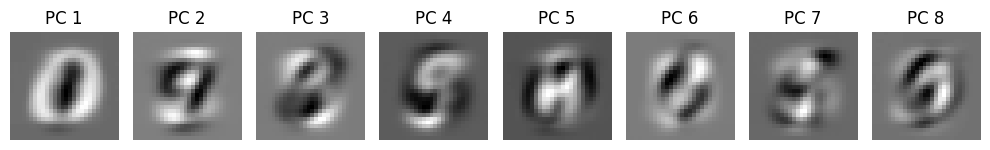
\includegraphics[width=0.5\textwidth]{pca.png}
    \caption{8-PCA plot}
\end{figure}

\textbf{4.} In this part i again trained same multilayer perceptron as in part 1 but used 50 PCA features as input and got ccuracy on test data : $\approx$ 95\% , for code refer \boxed{\texttt{AIML\_2025\_A2\_23684.py}}
\vspace{7pt}

\textbf{5.} In this part of the question i trained a logistic regression model for multiclass classification abd then train a model binary classifier \texttt{one\_vs\_rest()}

\item \textbf{Deliverables}

\textbf{1.} I reconstructed image of digit $8$ using different number of principal components

\begin{figure}[h]
    \centering
    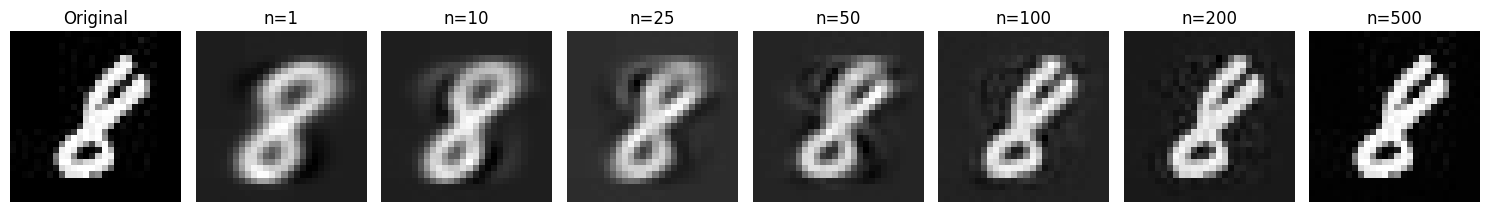
\includegraphics[width=0.8\textwidth]{pca8.png}
    \caption{Reconstructed image of digit 8}
\end{figure}
from the plot we can see that as we increase the number of principal components the image is getting clearer and clearer.
specifically when we use $100+$ the image is almost identical to the original image.

\textbf{3.} Here is the ROC plot for each class for \texttt{one\_vs\_rest()} classifier also average AUC i got is 0.88 
\begin{figure}[h]
    \centering
    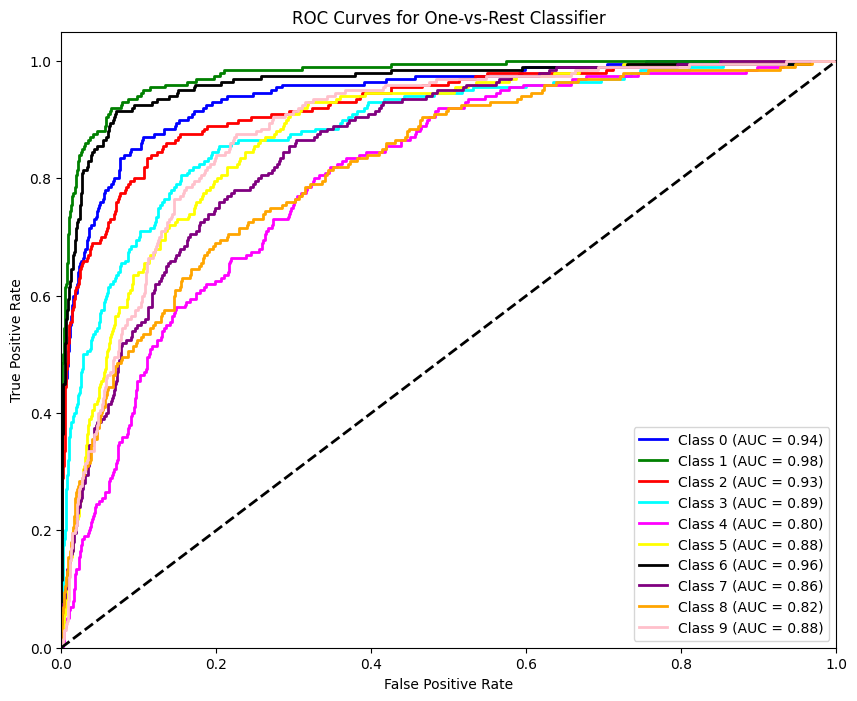
\includegraphics[width=0.8\textwidth]{aoc.png}
    \caption{ROC plot for each class}
\end{figure}

\newpage
\textbf{2.} Metrics for each model for each class as well are as follows

\begin{figure}[h]
    \centering
    \begin{minipage}{0.45\textwidth}
        \centering
        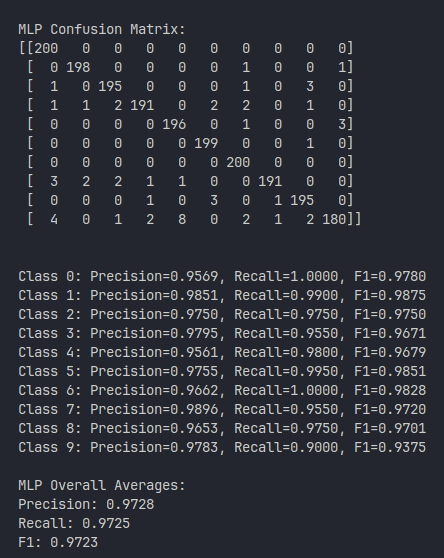
\includegraphics[width=\linewidth]{1.png}
    \end{minipage}
    \hfill
    \begin{minipage}{0.45\textwidth}
        \centering
        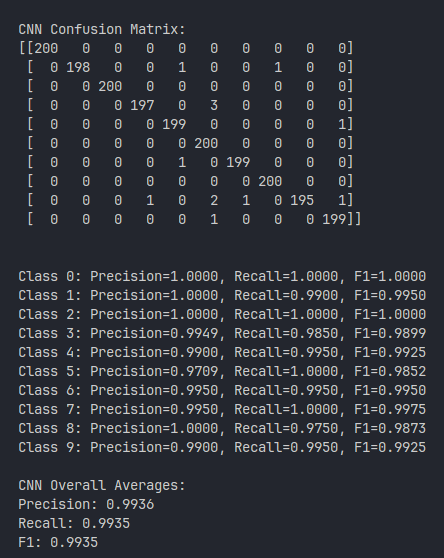
\includegraphics[width=\linewidth]{2.png}
    \end{minipage}

    \vspace{0.3cm}  % Adjust spacing between rows

    \begin{minipage}{0.45\textwidth}
        \centering
        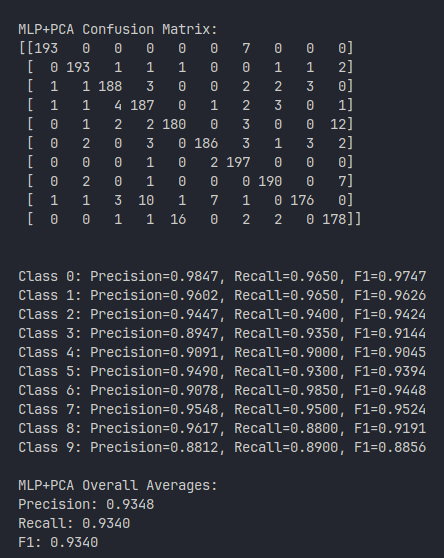
\includegraphics[width=\linewidth]{3.png}
    \end{minipage}
    \hfill
    \begin{minipage}{0.45\textwidth}
        \centering
        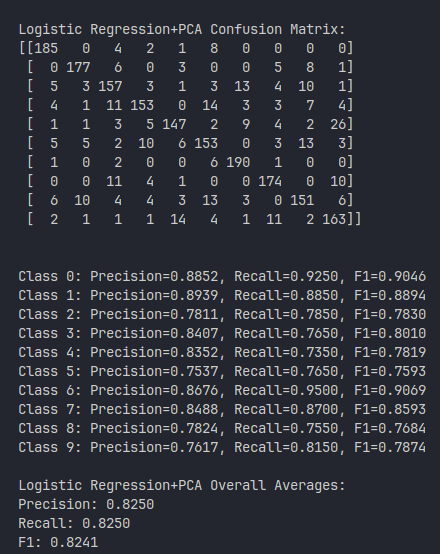
\includegraphics[width=\linewidth]{4.png}
    \end{minipage}
    
\end{figure}

\begin{itemize}
    \item Top Left image is for MLP model
    \item Top Right image is for CNN model
    \item Bottom Left image is for PCA + MLP model
    \item Bottom Right image is for Logistic Regression model
\end{itemize}


\end{itemize}
\newpage

\noindent    \textbf{Solution 3 : Regression}
\vspace{7pt}

\noindent $\circ$ \textbf{Linear Regression}

\begin{itemize}
    \item \textbf{Tasks}
    
    \textbf{1.} Query for data done in code! refer \boxed{\texttt{AIML\_2025\_A2\_23684.py}}

    \textbf{2.} Solved the linear regression and ridge regression problem using the given dataset $\mathcal{D}_1$ and $\mathcal{D}_2$ for $\lambda = 1$
    \begin{itemize}
        \item Ordinary least square regression
        \[
        \boxed{J(w) = \frac{1}{2n} \sum_{i=1}^{n} (y_i - w^T x_i)^2 = \frac{1}{2n} \|Y - Xw\|^2}
        \]
        \hspace{110pt} where $X \in \mathbb{R}^{n \times d}$ , $Y \in \mathbb{R}^{n}$ ,  $x^{(i)}, \in \mathbb{R}^d$ and $y^{(i)} \in \mathbb{R}$ 

        \item Ridge regression
        \[
        \boxed{J(w) = = \frac{1}{2n} \|Y - Xw\|^2 + \frac{\lambda}{2} \|w\|^2}
        \]
        \hspace{110pt} where $X \in \mathbb{R}^{n \times d}$ , $Y \in \mathbb{R}^{n}$ ,  $x^{(i)}, \in \mathbb{R}^d$ and $y^{(i)} \in \mathbb{R}$ 
        \vspace{7pt}

        while solving both problems i used \textbf{cvxopt} for convex optimization with $C=1$ 
    \end{itemize}


    \textbf{3.} MSE for $w_1^{ols},w_1^{rr}$ and $w_2^{ols},w_2^{rr}$ for dataset $\mathcal{D}_1$ and $\mathcal{D}_2$ are as follows
    \begin{itemize}
        \item For dataset $\mathcal{D}_1$
        \begin{itemize}
            \item Ordinary least square regression method : 0.058230037381664414
            \item Ridge regression method : 0.05123724209499151
        \end{itemize}
        For dataset $\mathcal{D}_2$ 
        \begin{itemize}
            \item Ordinary least square regression method : 65556.6898497358
            \item Ridge regression method : 10.748440456477965
        \end{itemize}
    \end{itemize}

    \item \textbf{Deliverables} 
    
        \textbf{1.} Final solution that we get for ordinary least square regression method is
        \[w = (X^TX)^{-1}X^T Y\]
        but if $X$ is not full rank then $(X^TX)^{-1}$ will not exist we can solve this problem by using ridge regression method or stochastic gradient descent method.\vspace{10pt} \\
        \textbf{2.} MSE results are mentioned above in task 3 and $w_1^{ols},w_1^{rr}$ are below
        \begin{itemize}
            \item $w_1^{ols} = [[-0.24396582],[-1.37368806],[ 0.192258012],
 [ 0.10943952],$ \\
            $[-0.05493344],[ 0.18603667],[ 0.69107121],[ 0.2482359 ],[ 0.08276927],[-0.0738674 ]]$ \vspace{7pt}
            \item $w_1^{rr} = [[-0.25445716],
 [-1.3052957 ],
 [ 0.28605436],
 [ 0.07646213],
 $ \\
 $[-0.09351605],
 [ 0.15510994],
 [ 0.63710072],
 [ 0.22491536],
 [ 0.06385936],
 [-0.08760024]]$
        \end{itemize}
    
    \textbf{3.} MSE results are mentioned above in task 3 and $w_2^{ols},w_2^{rr}$ are in \boxed{\texttt{w\_ols\_23684.csv}} , \boxed{\texttt{w\_rr\_23684.csv}} 

    \hspace{10pt} respectively which are attached in submission on teams.
\vspace{7pt}
\end{itemize}

\noindent $\circ$ \textbf{Support Vector Regression}
\begin{itemize}
    \item \textbf{Tasks}
    \vspace{5pt}

    \textbf{1.} Solved the dual slack support vector regression using \textbf{cvxopt} refer \boxed{\texttt{AIML\_2025\_A2\_23684.py}}

    \textbf{2.} Solved the dual kernelized support vector regression using \textbf{cvxopt} refer \boxed{\texttt{AIML\_2025\_A2\_23684.py}}

    \item \textbf{Deliverables :} Plot of predicted values , average values and actual  values for each $\gamma$ and $time$ are below
\end{itemize}
\newpage
\begin{figure}[h]
    \centering
    \renewcommand{\arraystretch}{2} % Adjust row spacing

    \setlength{\tabcolsep}{-25pt}
   \noindent \begin{tabular}{ccc} % 3 columns
        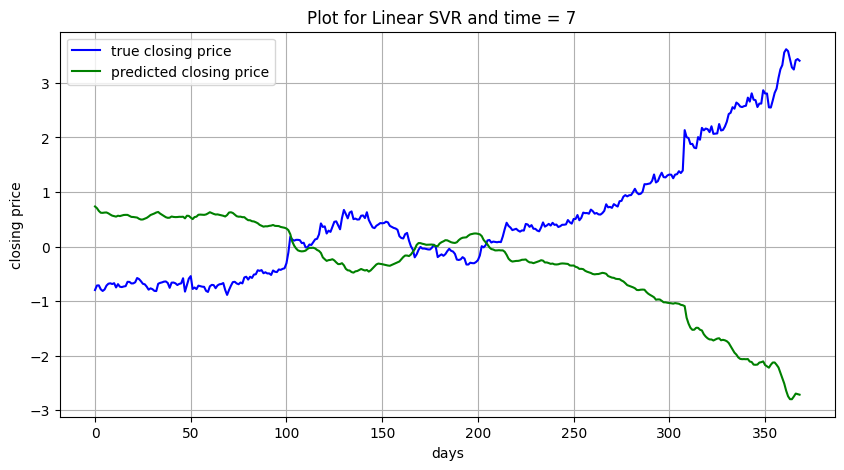
\includegraphics[width=0.45\textwidth]{linear7.png} &  
        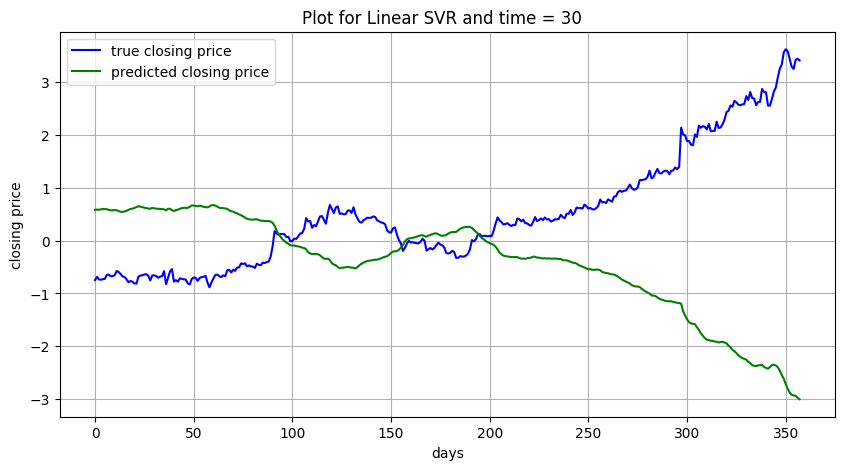
\includegraphics[width=0.45\textwidth]{linear30.png} &  
        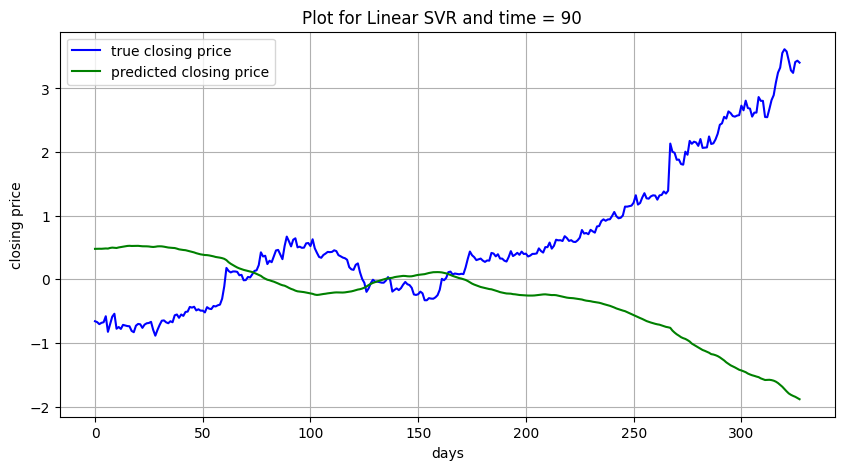
\includegraphics[width=0.45\textwidth]{linear90.png} \\

        \small Linear SVR (t=7) & \small Linear SVR (t=30) & \small Linear SVR (t=90) \\

        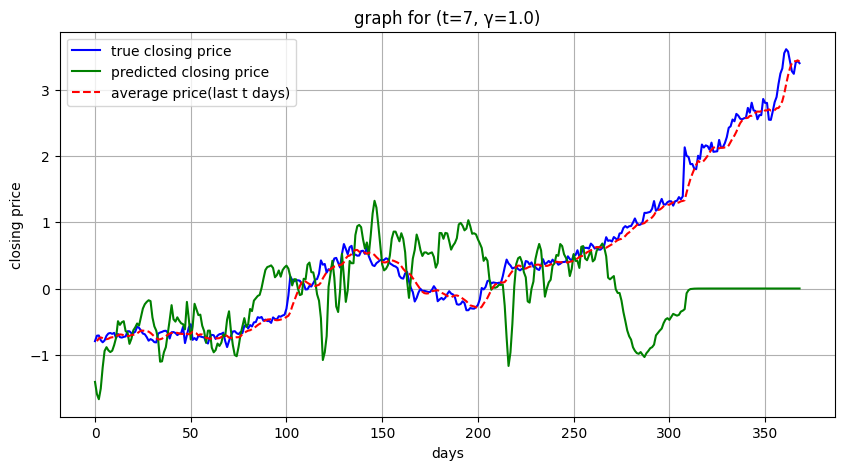
\includegraphics[width=0.45\textwidth]{kernel7_1.png} &  
        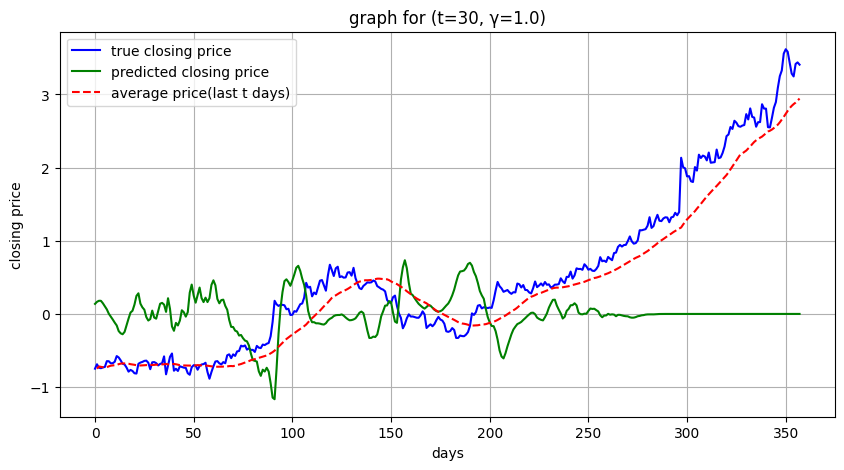
\includegraphics[width=0.45\textwidth]{kernel30_1.png} &  
        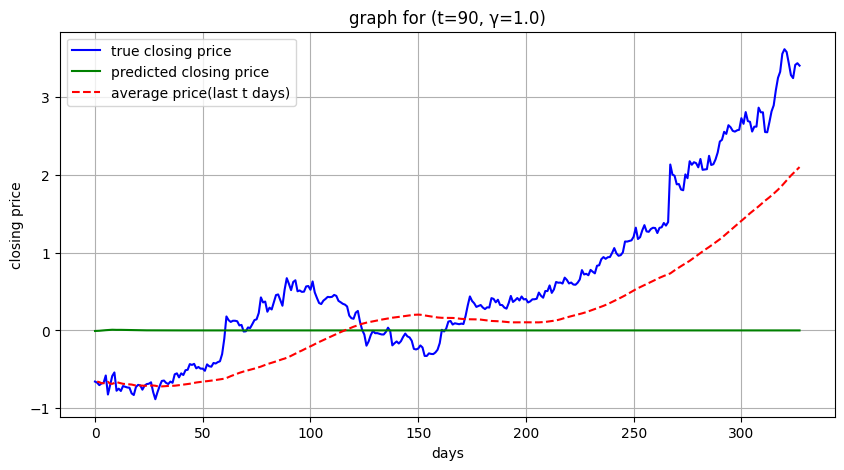
\includegraphics[width=0.45\textwidth]{kernel90_1.png} \\

        \small Kernel SVR (t=7, $\gamma=1$) & \small Kernel SVR (t=30, $\gamma=1$) & \small Kernel SVR (t=90, $\gamma=1$) \\

        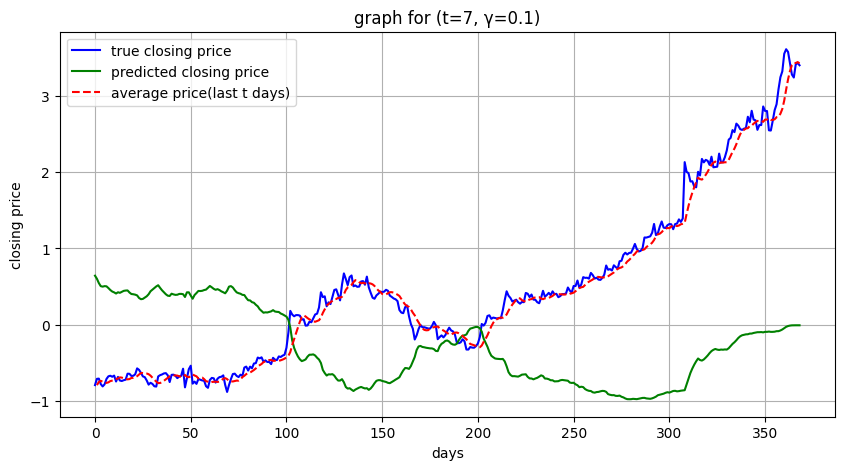
\includegraphics[width=0.45\textwidth]{kernel7_10.png} &  
        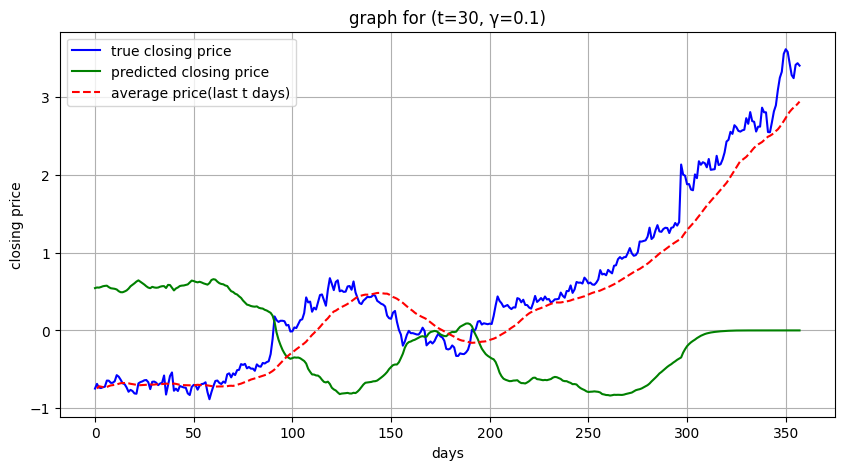
\includegraphics[width=0.45\textwidth]{kernel30_10.png} &  
        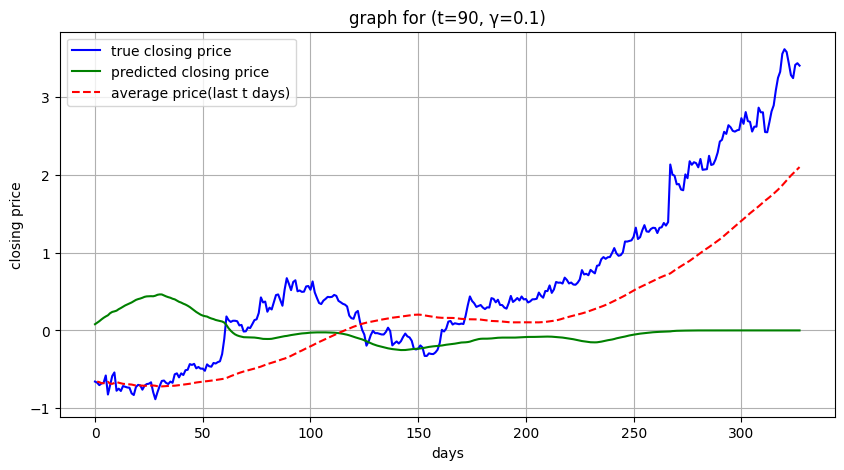
\includegraphics[width=0.45\textwidth]{kernel90_10.png} \\

        \small Kernel SVR (t=7, $\gamma=0.1$) & \small Kernel SVR (t=30, $\gamma=0.1$) & \small Kernel SVR (t=90, $\gamma=0.1$) \\

        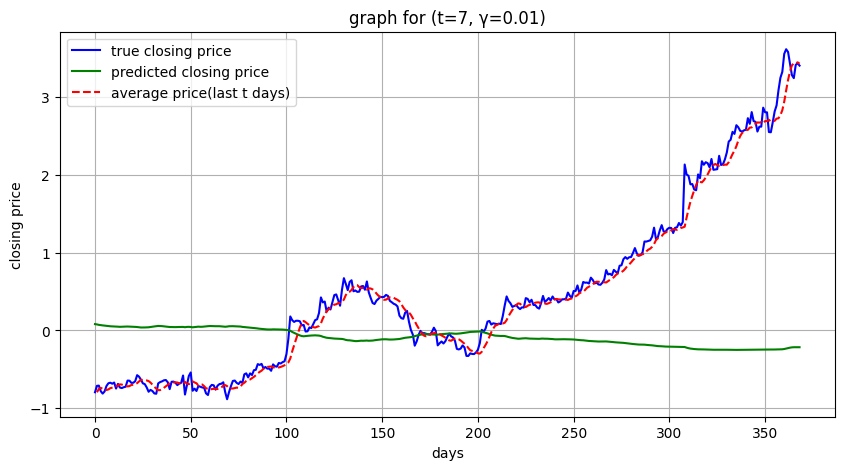
\includegraphics[width=0.45\textwidth]{kernel7_100.png} &  
        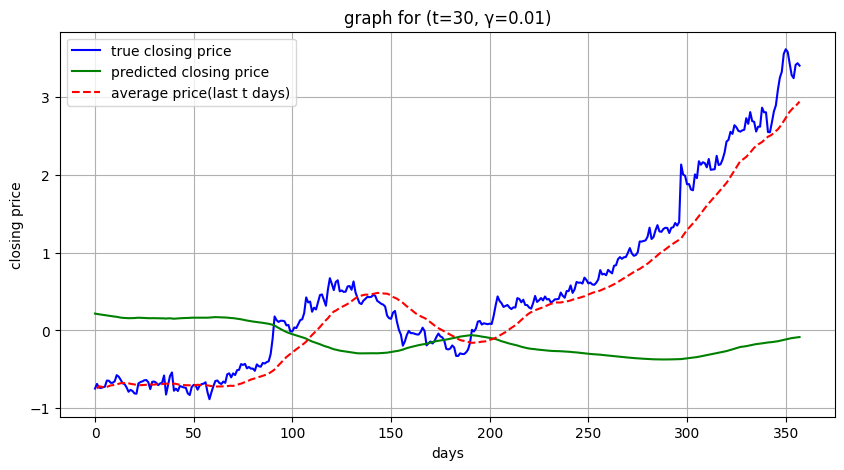
\includegraphics[width=0.45\textwidth]{kernel30_100.png} &  
        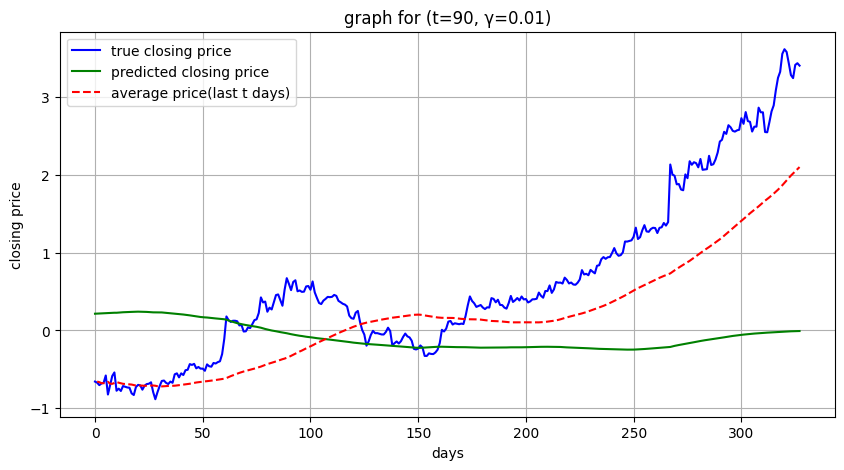
\includegraphics[width=0.45\textwidth]{kernel90_100.png} \\

        \small Kernel SVR (t=7, $\gamma=0.01$) & \small Kernel SVR (t=30, $\gamma=0.01$) & \small Kernel SVR (t=90, $\gamma=0.01$) \\

        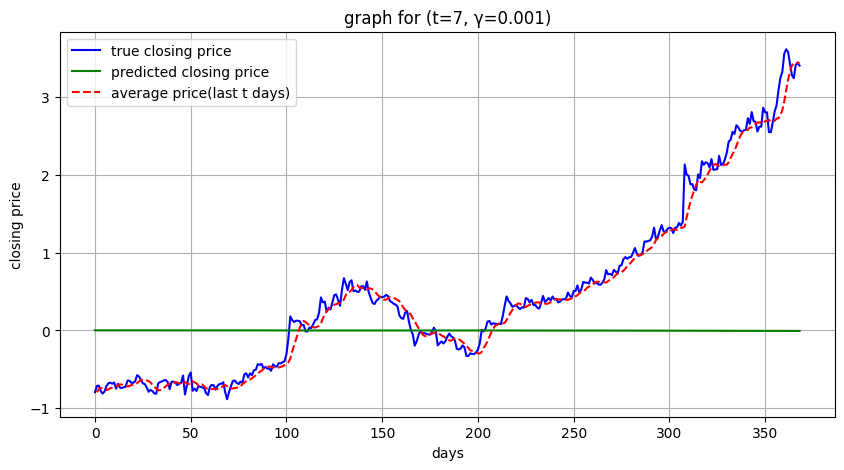
\includegraphics[width=0.45\textwidth]{kernel7_1000.png} &  
        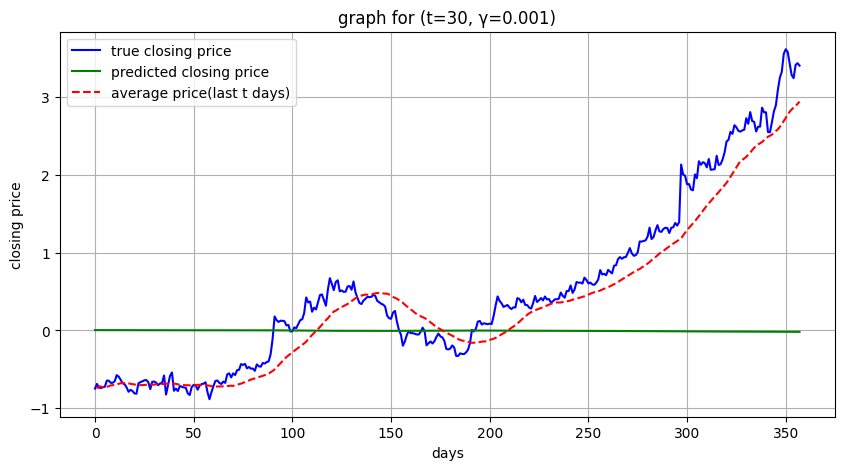
\includegraphics[width=0.45\textwidth]{kernel30_1000.png} &  
        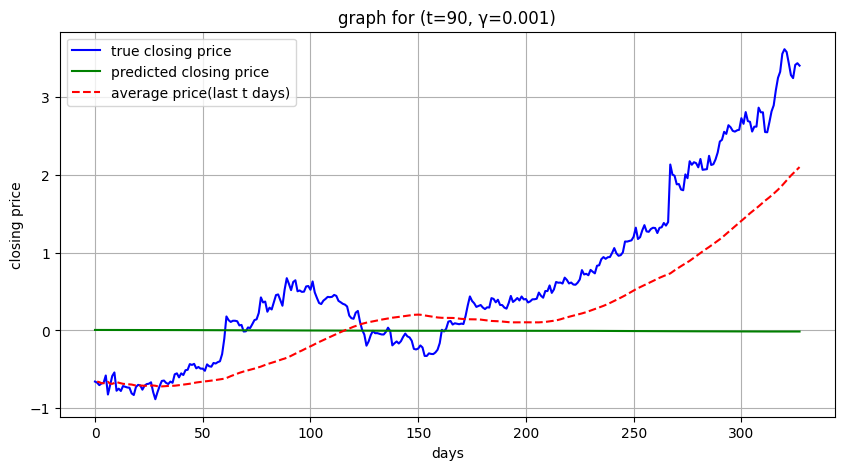
\includegraphics[width=0.45\textwidth]{kernel90_1000.png} \\

        \small Kernel SVR (t=7, $\gamma=0.001$) & \small Kernel SVR (t=30, $\gamma=0.001$) & \small Kernel SVR (t=90, $\gamma=0.001$) \\
    \end{tabular}
\end{figure}


\end{document}